\documentclass[dvisvgm, tikz]{standalone}
\usepackage{tikz}
\usetikzlibrary{automata, positioning, arrows.meta, calc}

\begin{document}
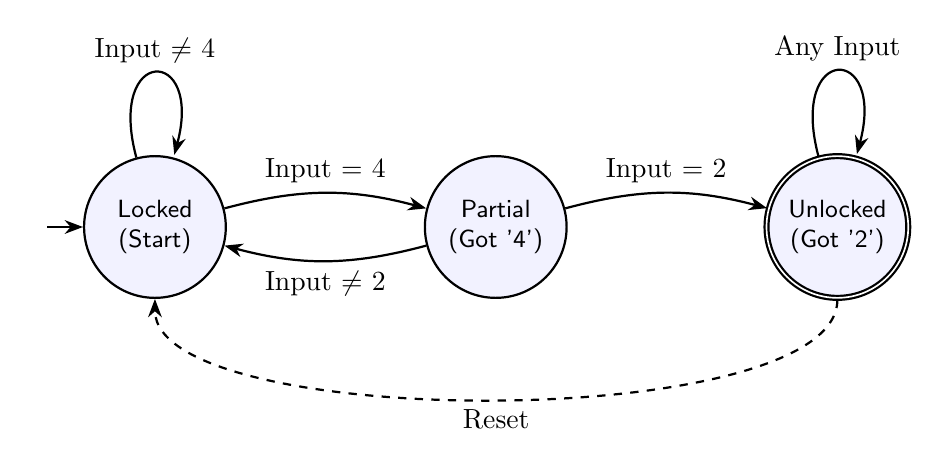
\begin{tikzpicture}[
    ->, >=Stealth, auto,
    node distance=2.5cm,
    line width=0.8pt,
    every state/.style={
        draw=black, 
        thick, 
        fill=blue!5, 
        minimum size=1.8cm,
        font=\sffamily\small,
        align=center
    },
    initial text={},
    every edge/.style={draw, thick}
]

    % States
    \node[state, initial] (S0) {Locked\\(Start)};
    \node[state, right=of S0] (S1) {Partial\\(Got '4')};
    \node[state, right=of S1, accepting] (S2) {Unlocked\\(Got '2')};

    % Transitions
    % S0 transitions
    \path (S0) edge[loop above] node {Input $\neq$ 4} (S0)
               edge[bend left=15] node[above] {Input = 4} (S1);

    % S1 transitions
    \path (S1) edge[bend left=15] node[below] {Input $\neq$ 2} (S0)
               edge[bend left=15] node[above] {Input = 2} (S2);

    % S2 transitions (Reset logic)
    \path (S2) edge[loop above] node {Any Input} (S2);
    
    % Add a "Reset" arrow back to start for visual completeness effectively
    \draw [dashed, ->] (S2) to[out=270,in=270, looseness=0.5] node[below] {Reset} (S0);

\end{tikzpicture}
\end{document}
